% ============================================================
%  EchoBreaker — UNESCO Youth MIL Hackathon 2026
%  Project Proposal
% ============================================================

\documentclass[11pt, a4paper]{article}

% ── Packages ─────────────────────────────────────────────────
\usepackage[T1]{fontenc}
\usepackage[utf8]{inputenc}
\usepackage[english]{babel}
\usepackage{lmodern}
\usepackage{microtype}
\usepackage{geometry}
\usepackage{graphicx}
\usepackage{xcolor}
\usepackage{hyperref}
\usepackage{titlesec}
\usepackage{enumitem}
\usepackage{tabularx}
\usepackage{booktabs}
\usepackage{fancyhdr}
\usepackage{mdframed}
\usepackage{multicol}
\usepackage{tcolorbox}
\usepackage{array}
\usepackage{parskip}
\usepackage{fontawesome5}
\usepackage{amsmath}
\usepackage{caption}
\usepackage{tikz}
\usepackage{needspace}
\usetikzlibrary{shapes.geometric, arrows.meta, positioning, fit, calc}

% ── Page geometry ────────────────────────────────────────────
\geometry{
  top    = 2.0cm,
  bottom = 2.0cm,
  left   = 2.2cm,
  right  = 2.2cm,
  headheight = 28pt
}

% ── Colour palette ────────────
\definecolor{echored}{HTML}{A8412E}
\definecolor{echogold}{HTML}{B8862E}
\definecolor{echoink}{HTML}{1C1B1A}
\definecolor{echogreen}{HTML}{5C7A6B}
\definecolor{echobg}{HTML}{F5F0EB}
\definecolor{echoborder}{HTML}{D9D3CB}
\definecolor{echomuted}{HTML}{5C5750}

% ── Hyperref setup ───────────────────────────────────────────
\hypersetup{
  colorlinks = true,
  linkcolor  = echored,
  urlcolor   = echored,
  citecolor  = echored,
  pdftitle   = {EchoBreaker -- UNESCO Youth MIL Hackathon 2026 Proposal},
  pdfauthor  = {Benouali Abdelkader, BENDJERIOU SEDJERARI Abdellah}
}

% ── Section styling ──────────────────────────────────────────
\titleformat{\section}
  {\large\bfseries\color{echored}}
  {\thesection.}{0.6em}{}
  [\vspace{-4pt}\textcolor{echoborder}{\rule{\linewidth}{0.5pt}}]

\titleformat{\subsection}
  {\normalsize\bfseries\color{echoink}}
  {\thesubsection.}{0.5em}{}

\titlespacing{\section}{0pt}{12pt}{4pt}
\titlespacing{\subsection}{0pt}{8pt}{3pt}

% ── Header / Footer ──────────────────────────────────────────
\pagestyle{fancy}
\fancyhf{}
\fancyhead[L]{\small\textcolor{echomuted}{\textbf{EchoBreaker} --- UNESCO Youth MIL Hackathon 2026}}
\fancyhead[R]{\small\textcolor{echomuted}{Algeria}}
\fancyfoot[C]{\small\textcolor{echomuted}{\thepage}}
\renewcommand{\headrulewidth}{0.4pt}
\renewcommand{\headrule}{\hbox to\headwidth{\color{echoborder}\leaders\hrule height \headrulewidth\hfill}}

% ── Custom box environments ───────────────────────────────────
\tcbuselibrary{skins, breakable}

\newtcolorbox{criteriabox}[2][]{
  enhanced, breakable=false,
  colback      = echobg,
  colframe     = echored,
  colbacktitle = echored,
  coltitle     = white,
  fonttitle    = \bfseries\small,
  title        = {#2},
  left=8pt, right=8pt, top=6pt, bottom=6pt,
  arc=4pt,
  #1
}

\newtcolorbox{honestbox}[1][]{
  enhanced, breakable=false,
  colback  = echobg,
  colframe = echogold,
  left=8pt, right=8pt, top=5pt, bottom=5pt,
  arc=4pt,
  #1
}

% ── List settings ────────────────────────────────────────────
\setlist[itemize]{leftmargin=1.4em, itemsep=2pt, topsep=3pt}
\setlist[enumerate]{leftmargin=1.4em, itemsep=2pt, topsep=3pt}

% ═════════════════════════════════════════════════════════════
\begin{document}

% ── COVER PAGE ───────────────────────────────────────────────
\thispagestyle{empty}
\begin{center}

  \vspace*{0.6cm}
  
  % ACTUAL WEBSITE LOGO RECREATION
  
\begin{tikzpicture}
    \node (mark) [draw=none, fill=echored, rounded corners=6pt, minimum size=42pt, inner sep=0pt] {
      \textcolor{white}{\fontsize{20}{20}\selectfont\bfseries EB}
    };
  \end{tikzpicture}
  \vspace{0.35cm}

  {\fontsize{36}{40}\selectfont
    \textbf{\textcolor{echoink}{ECHO}\textcolor{echored}{BREAKER}}}

  \vspace{0.3cm}
  {\large\itshape\textcolor{echomuted}{Teaching Algorithmic Literacy Through Radical Transparency}}

  \vspace{0.8cm}
  \textcolor{echoborder}{\rule{0.65\textwidth}{0.8pt}}
  \vspace{0.4cm}

  {\normalsize
    \begin{tabular}{rl}
      \textbf{Hackathon:}  & UNESCO Youth Media and Information Literacy Hackathon 2026\\[4pt]
      \textbf{Project Name:} & EchoBreaker \\[4pt]
      \textbf{Team Name:}  & Team EchoBreaker \\[4pt]
      \textbf{Selected Track:} & AI and Media and Information Literacy (MIL) \\[4pt]
      \textbf{Project Format:} & Interactive Digital Learning Tool (Browser-based app)\\[4pt]
      \textbf{Submission Date:} & 08 August 2026 \\
    \end{tabular}
  }

  \vspace{0.8cm}
  \textcolor{echoborder}{\rule{0.65\textwidth}{0.8pt}}
  \vspace{0.4cm}

  {\normalsize
    \textbf{Team Members}\\[8pt]
    \renewcommand{\arraystretch}{1.3}
    \begin{tabular}{llcc}
      \textbf{Name} & \textbf{Role} & \textbf{Country} & \textbf{Age} \\
      \midrule
      Benouali Abdelkader & Developer & Algeria & 22 \\
      BENDJERIOU SEDJERARI Abdellah & Designer & Algeria & 23 \\
    \end{tabular}
  }

  \vspace{0.8cm}
  \textcolor{echoborder}{\rule{0.65\textwidth}{0.8pt}}

\end{center}

\newpage
\pagenumbering{arabic}

% ── TABLE OF CONTENTS & LIST OF FIGURES (1 SINGLE PAGE) ────────
\begin{center}
  {\large\bfseries\color{echored} Table of Contents \& Index of Figures}
\end{center}
\vspace{-4pt}

\tableofcontents

\vspace{12pt}
\textcolor{echoborder}{\rule{\linewidth}{0.5pt}}
\vspace{6pt}

\phantomsection
\addcontentsline{toc}{section}{List of Figures}
\listoffigures

\newpage

% ═════════════════════════════════════════════════════════════
\section{Executive Summary}

EchoBreaker is an open-access, browser-based educational tool designed to combat epistemic polarisation by teaching algorithmic literacy to youth. While most MIL curricula focus on \emph{what} misinformation is, EchoBreaker teaches \emph{why} it spreads by allowing students to experience algorithmic echo chambers in real-time. Through four interconnected modules (Feed Simulator, Echo Escape Arena, Agency Toolkit, and Impact Command Center), users uncover how recommendation systems prioritize engagement over truth. Built primarily in English for universal hackathon evaluation and international accessibility, EchoBreaker features a modular i18n architecture ready for zero-code translation into Arabic, French, and local languages. Our solution ensures zero-install, low-bandwidth adoption to equip youth with the critical framework needed to navigate digital feeds.

% ═════════════════════════════════════════════════════════════
\section{The Team}

\begin{center}
\renewcommand{\arraystretch}{1.2}
\begin{tabularx}{\textwidth}{p{4.8cm} p{3.8cm} X l c}
\toprule
\textbf{Name} & \textbf{Role} & \textbf{Core Expertise} & \textbf{Country} & \textbf{Age} \\
\midrule
Benouali Abdelkader & Lead Developer & Vanilla JS, Scoring Engine & Algeria & 22 \\
BENDJERIOU SEDJERARI Abdellah & Designer \& Pedagogical Lead & UI/UX Design, Curriculum & Algeria & 23 \\
\bottomrule
\end{tabularx}
\end{center}

\textbf{Why this team?} We combine technical software engineering with visual UI/UX design and pedagogical content structuring. Benouali architects lightweight, zero-dependency code optimized for low-spec devices, while BENDJERIOU SEDJERARI ensures intuitive visual ergonomics and alignment with educational standards. The team collaborates with secondary school educators to validate classroom feasibility.

% ═════════════════════════════════════════════════════════════
\section{Problem Statement}

For the estimated \textbf{5.79 billion} social media user identities worldwide (DataReportal 2026)---the majority under 30---recommendation algorithms operate invisibly. The logic governing feed ranking remains unexamined, fostering filter bubbles, epistemic polarisation, and emotional manipulation.

Existing Media and Information Literacy (MIL) curricula predominantly address \emph{what} misinformation is, failing to expose \emph{why} it spreads. The AI-driven mathematical, architectural, and attentional systems that amplify content regardless of factual quality remain black boxes. With AI-generated content accelerating online noise, fact-checking alone is insufficient without a structural understanding of algorithmic amplification.

% ═════════════════════════════════════════════════════════════
\section{Objectives \& Contingency Plan}

\textbf{Main SMART Objective:}\\
By Q4 2026, launch a phased pilot across 5 initial partner schools (150 students), scaling to 50 secondary schools and 1,500 youth by Q2 2027, achieving a verified 70\% increase in algorithmic literacy measured via pre/post-session comprehension checks and behavioral pledges.

\textbf{Supporting Operational Objectives:}
\begin{itemize}
    \item \textbf{Global \& Local Tool Deployment:} Maintain a zero-install, 100\% English core tool with instant i18n localization hooks for Arabic and French regional adaptation.
    \item \textbf{Facilitate Educators:} Provide zero-setup Teacher Facilitation Guides and printable offline toolkits (\texttt{print-game.html}, \texttt{print-report.html}) enabling seamless 30-minute MIL lessons.
\end{itemize}

\textbf{Contingency Strategy (Plan B):} If formal school onboarding experiences administrative delay or bandwidth limits, EchoBreaker deploys through offline printable worksheets and peer-to-peer UNESCO Youth Ambassador networks.

% ═════════════════════════════════════════════════════════════
\section{Target Audience}

Our primary target audience consists of \textbf{Secondary students (ages 14--18)} and global youth learners. 

\textbf{Why this audience?} Youth are actively forming long-term digital habits and online identities, making them highly vulnerable to algorithmic polarization.

\textbf{How will we reach them?} Through school partnerships, UNESCO youth workshops, and civil society networks. Built in lightweight Vanilla JS, EchoBreaker guarantees low-bandwidth accessibility for marginalized and underserved youth on low-end devices. Multi-language i18n support ensures local language readiness for North African, Middle Eastern, and global classrooms.

% ═════════════════════════════════════════════════════════════
% ═════════════════════════════════════════════════════════════
\section{Proposed Solution / Concept \& Prototype}

EchoBreaker is structured around four interconnected modules enacting UNESCO's MIL \textbf{4A Framework} (Algorithm, Amplification, Attention, Agency). Interface screenshots are paired directly with algorithmic flow diagrams:

\begin{figure}[htpb]
    \centering
    \vspace{-4pt}
    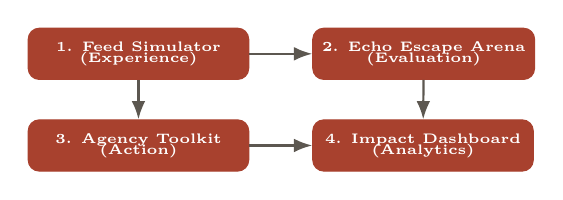
\begin{tikzpicture}[
        arrow/.style={-Latex, thick, echomuted},
        module/.style={draw, rounded corners=4pt, minimum width=2.8cm, minimum height=0.65cm, align=center, font=\tiny\bfseries, fill=echored, text=white, draw=echored}
    ]
        \node (feed) [module] {1. Feed Simulator\\[-2pt]\tiny(Experience)};
        \node (game) [module, right=0.8cm of feed] {2. Echo Escape Arena\\[-2pt]\tiny(Evaluation)};
        \node (toolkit) [module, below=0.5cm of feed] {3. Agency Toolkit\\[-2pt]\tiny(Action)};
        \node (dashboard) [module, right=0.8cm of toolkit] {4. Impact Dashboard\\[-2pt]\tiny(Analytics)};
        
        \draw [arrow] (feed) -- (game);
        \draw [arrow] (game) -- (dashboard);
        \draw [arrow] (feed) -- (toolkit);
        \draw [arrow] (toolkit) -- (dashboard);
    \end{tikzpicture}
    \vspace{-6pt}
    \caption{Diagram 1: System Flow \& Module Architecture.}
    \label{fig:architecture}
\end{figure}

\vspace{-4pt}
\subsection{Module Breakdown: Interfaces \& Algorithmic Logic}

% ── MODULE 1 PAIR ─────────────────────────────────────────────
\noindent
\begin{minipage}[c]{0.43\textwidth}
    \centering
    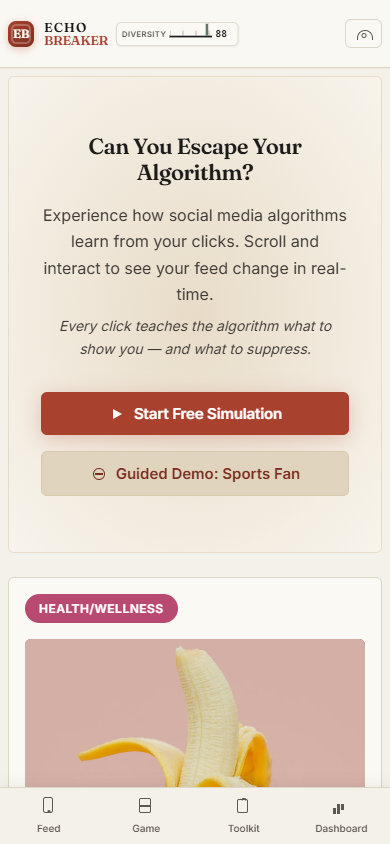
\includegraphics[height=5.0cm, keepaspectratio]{feed_screenshot.png}
    \captionof{figure}{Module 1: Feed Simulator}
    \label{fig:feed_ui}
\end{minipage}\hfill
\begin{minipage}[c]{0.54\textwidth}
    \textbf{1. Feed Simulator (The Experience):}\par\smallskip
    Students explore an algorithmically ranked feed. As they scroll and like, posts re-rank instantly. Dwell time is tracked via \texttt{IntersectionObserver}.
    
    \vspace{4pt}
    \centering
    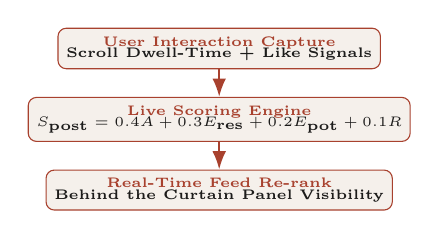
\begin{tikzpicture}[
        box/.style={draw=echored, fill=echobg, rounded corners=3pt, font=\tiny\bfseries, align=center, inner sep=3pt, text=echoink, minimum width=3.8cm},
        arrow/.style={-Latex, thick, echored}
    ]
        \node (user) [box] {\textcolor{echored}{User Interaction Capture}\\[-2pt]\tiny Scroll Dwell-Time + Like Signals};
        \node (engine) [box, below=0.35cm of user] {\textcolor{echored}{Live Scoring Engine}\\[-2pt]\tiny $S_{\text{post}} = 0.4A + 0.3E_{\text{res}} + 0.2E_{\text{pot}} + 0.1R$};
        \node (rerank) [box, below=0.35cm of engine] {\textcolor{echored}{Real-Time Feed Re-rank}\\[-2pt]\tiny Behind the Curtain Panel Visibility};
        
        \draw [arrow] (user) -- (engine);
        \draw [arrow] (engine) -- (rerank);
    \end{tikzpicture}
    \captionof{figure}{Diagram 2: Module 1 Engine Logic.}
    \label{fig:diag_feed}
\end{minipage}

\vspace{6pt}

% ── MODULE 2 PAIR ─────────────────────────────────────────────
\noindent
\begin{minipage}[c]{0.43\textwidth}
    \centering
    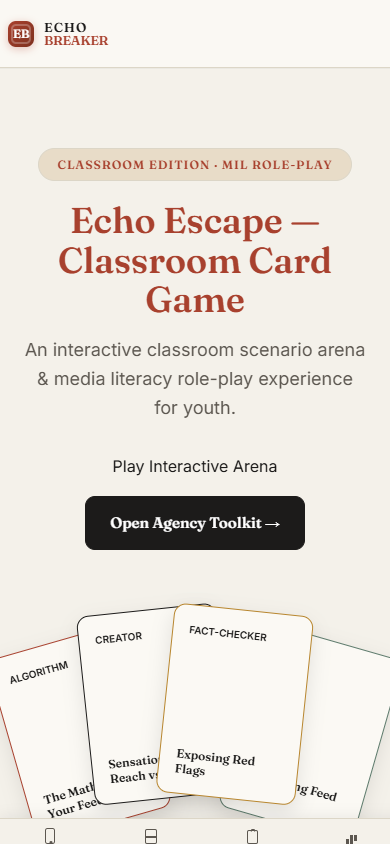
\includegraphics[height=5.0cm, keepaspectratio]{game_screenshot.png}
    \captionof{figure}{Module 2: Echo Escape Arena}
    \label{fig:game_ui}
\end{minipage}\hfill
\begin{minipage}[c]{0.54\textwidth}
    \textbf{2. Echo Escape Arena (The Evaluation):}\par\smallskip
    An interactive 12-card scenario arena where students adopt roles (Algorithm, Content Creator, Fact-Checker) and evaluate headlines as Credible or Misleading \emph{before} red flags and XP debriefs unlock.
    
    \vspace{4pt}
    \centering
    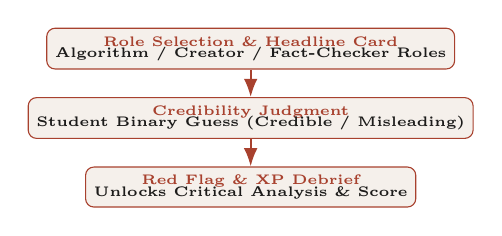
\begin{tikzpicture}[
        box/.style={draw=echored, fill=echobg, rounded corners=3pt, font=\tiny\bfseries, align=center, inner sep=3pt, text=echoink, minimum width=3.8cm},
        arrow/.style={-Latex, thick, echored}
    ]
        \node (card) [box] {\textcolor{echored}{Role Selection \& Headline Card}\\[-2pt]\tiny Algorithm / Creator / Fact-Checker Roles};
        \node (guess) [box, below=0.35cm of card] {\textcolor{echored}{Credibility Judgment}\\[-2pt]\tiny Student Binary Guess (Credible / Misleading)};
        \node (reveal) [box, below=0.35cm of guess] {\textcolor{echored}{Red Flag \& XP Debrief}\\[-2pt]\tiny Unlocks Critical Analysis \& Score};
        
        \draw [arrow] (card) -- (guess);
        \draw [arrow] (guess) -- (reveal);
    \end{tikzpicture}
    \captionof{figure}{Diagram 3: Module 2 Role-Play Evaluation Mechanics.}
    \label{fig:diag_game}
\end{minipage}

\vspace{10pt}

% ── MODULE 3 PAIR ─────────────────────────────────────────────
\noindent
\begin{minipage}[c]{0.43\textwidth}
    \centering
    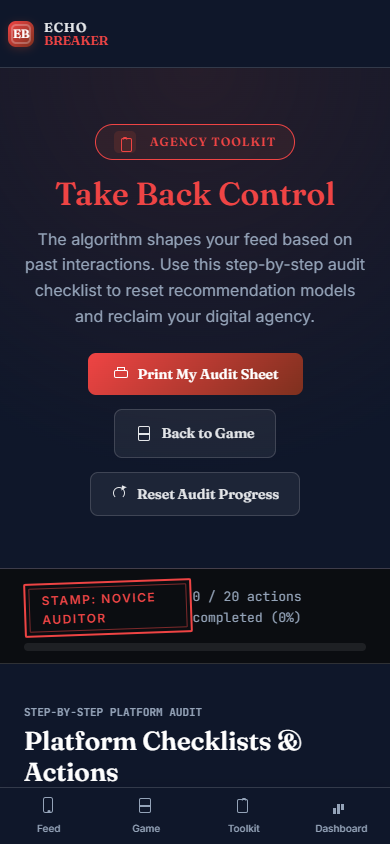
\includegraphics[height=5.4cm, keepaspectratio]{toolkit_screenshot.png}
    \captionof{figure}{Module 3: Agency Toolkit}
    \label{fig:toolkit_ui}
\end{minipage}\hfill
\begin{minipage}[c]{0.54\textwidth}
    \textbf{3. Agency Toolkit (The Action):}\par\smallskip
    A 20-item interactive audit checklist providing platform-specific actions (TikTok, YouTube, Meta) to reset recommendation models and restore digital autonomy.
    
    \vspace{4pt}
    \centering
    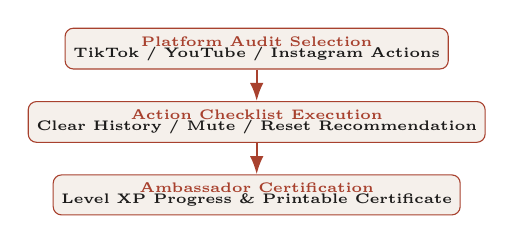
\begin{tikzpicture}[
        box/.style={draw=echored, fill=echobg, rounded corners=3pt, font=\tiny\bfseries, align=center, inner sep=3pt, text=echoink, minimum width=3.8cm},
        arrow/.style={-Latex, thick, echored}
    ]
        \node (platform) [box] {\textcolor{echored}{Platform Audit Selection}\\[-2pt]\tiny TikTok / YouTube / Instagram Actions};
        \node (action) [box, below=0.4cm of platform] {\textcolor{echored}{Action Checklist Execution}\\[-2pt]\tiny Clear History / Mute / Reset Recommendation};
        \node (cert) [box, below=0.4cm of action] {\textcolor{echored}{Ambassador Certification}\\[-2pt]\tiny Level XP Progress \& Printable Certificate};
        
        \draw [arrow] (platform) -- (action);
        \draw [arrow] (action) -- (cert);
    \end{tikzpicture}
    \captionof{figure}{Diagram 4: Module 3 Audit Pipeline.}
    \label{fig:diag_toolkit}
\end{minipage}

\vspace{8pt}

% ── MODULE 4 PAIR ─────────────────────────────────────────────
\noindent
\begin{minipage}[c]{0.43\textwidth}
    \centering
    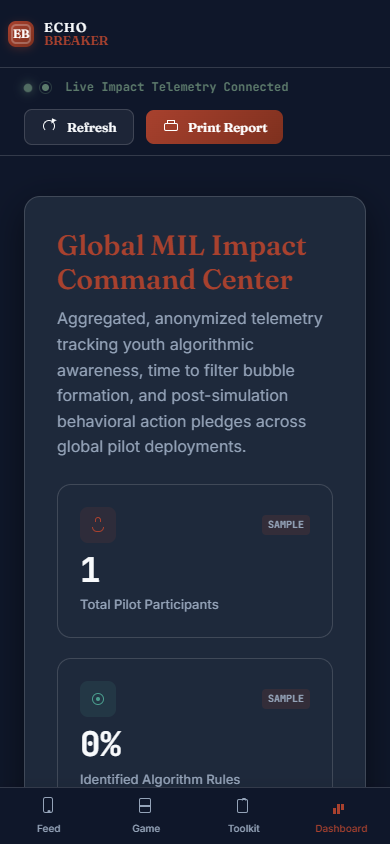
\includegraphics[height=5.4cm, keepaspectratio]{dashboard_screenshot.png}
    \captionof{figure}{Module 4: Impact Command Center}
    \label{fig:dashboard_ui}
\end{minipage}\hfill
\begin{minipage}[c]{0.54\textwidth}
    \textbf{4. Impact Command Center (The Analytics):}\par\smallskip
    An aggregate analytics dashboard for educators to visualize cohort telemetry, tracking time-to-echo-chamber and behavioral pledges without PII.
    
    \vspace{4pt}
    \centering
    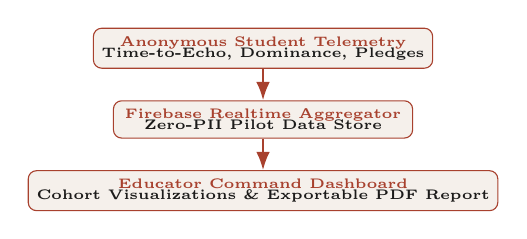
\begin{tikzpicture}[
        box/.style={draw=echored, fill=echobg, rounded corners=3pt, font=\tiny\bfseries, align=center, inner sep=3pt, text=echoink, minimum width=3.8cm},
        arrow/.style={-Latex, thick, echored}
    ]
        \node (telemetry) [box] {\textcolor{echored}{Anonymous Student Telemetry}\\[-2pt]\tiny Time-to-Echo, Dominance, Pledges};
        \node (firebase) [box, below=0.4cm of telemetry] {\textcolor{echored}{Firebase Realtime Aggregator}\\[-2pt]\tiny Zero-PII Pilot Data Store};
        \node (analytics) [box, below=0.4cm of firebase] {\textcolor{echored}{Educator Command Dashboard}\\[-2pt]\tiny Cohort Visualizations \& Exportable PDF Report};
        
        \draw [arrow] (telemetry) -- (firebase);
        \draw [arrow] (firebase) -- (analytics);
    \end{tikzpicture}
    \captionof{figure}{Diagram 5: Module 4 Telemetry Pipeline.}
    \label{fig:diag_dashboard}
\end{minipage}

\vspace{12pt}

\textbf{User Journey:} The student explores the feed. Once their feed diversity drops below 35\% ($D < 0.35$), a trigger pauses the experience, showing them how fast an echo chamber forms. They engage in the Arena role-play to evaluate content credibility and complete the Toolkit checklist to pledge behavioral actions.

\textbf{Direct Connection to UNESCO MIL 4A Framework:}
EchoBreaker directly enacts all four UNESCO MIL pillars:
\begin{itemize}[noitemsep,topsep=2pt]
    \item \textbf{Algorithm:} The live Behind the Curtain panel exposes real-time post scoring $S_{\text{post}}$.
    \item \textbf{Amplification:} Demonstrates how emotional tone ($E_{\text{res}}$) and engagement potential ($E_{\text{pot}}$) mathematically accelerate content reach regardless of factual accuracy.
    \item \textbf{Attention:} Uses 2-second dwell-time tracking via \texttt{IntersectionObserver} to reveal how passive scrolling trains recommendation algorithms.
    \item \textbf{Agency:} Empowers learners with platform audit checklists and verifiable action pledges to regain algorithmic control.
\end{itemize}

% ═════════════════════════════════════════════════════════════
\section{Innovation \& Creativity}

\begin{criteriabox}{Core Differentiator --- The Meta-Audit}
EchoBreaker uses \textbf{the same persuasive techniques it teaches students to resist}.
Glowing achievement badges, 3D card-flip animations, XP progress bars, and dopamine-reward unlocks are all deliberately present.

The reflection section explicitly reveals this contradiction:
\begin{quote}
\itshape
``Did you notice the glowing badges and 3D animations? We intentionally used \textbf{standard persuasive design (gamification)} to keep you engaged while teaching you how to resist it. How does it feel to recognise these emotional triggers working on you \emph{right now}?''
\end{quote}
\end{criteriabox}

This \textbf{Meta-Audit} is our central design innovation. The contradiction is the lesson. Live scoring transparency and dwell-time simulation using \texttt{IntersectionObserver} provide a technical realism rarely seen in educational tools, operating without heavy backend infrastructure.

% ═════════════════════════════════════════════════════════════
\section{Feasibility \& Sustainability}

\textbf{Tech Stack \& Architecture:} Built using pure HTML5, Vanilla JavaScript, and CSS. The zero-dependency frontend ensures zero supply-chain vulnerabilities, zero build tool breaking changes, and maximum long-term operational stability. Live hosting is deployed via Render static services (\url{https://echobreaker-mil.onrender.com}) backed by automated Blueprint configuration (\texttt{render.yaml}). Anonymous aggregate telemetry uses Firebase Realtime Database (free tier supports up to 100 concurrent connections, managed via client-side batching and local caching to easily accommodate classroom cohorts at \textbf{\$0 monthly cost}).

\begin{figure}[htpb]
    \centering
    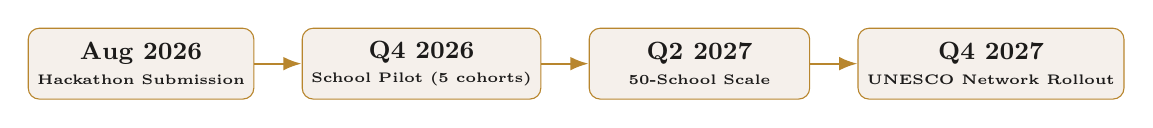
\begin{tikzpicture}[
        stage/.style={draw, rounded corners=4pt, minimum width=2.8cm, minimum height=0.9cm, align=center, font=\small\bfseries, fill=echobg, draw=echogold, text=echoink},
        arrow/.style={-Latex, thick, echogold}
    ]
        \node (s1) [stage] {Aug 2026\\[-2pt]\tiny Hackathon Submission};
        \node (s2) [stage, right=0.6cm of s1] {Q4 2026\\[-2pt]\tiny School Pilot (5 cohorts)};
        \node (s3) [stage, right=0.6cm of s2] {Q2 2027\\[-2pt]\tiny 50-School Scale};
        \node (s4) [stage, right=0.6cm of s3] {Q4 2027\\[-2pt]\tiny UNESCO Network Rollout};
        
        \draw [arrow] (s1) -- (s2);
        \draw [arrow] (s2) -- (s3);
        \draw [arrow] (s3) -- (s4);
    \end{tikzpicture}
    \caption{Diagram 6: Feasibility \& Phased Deployment Roadmap.}
    \label{fig:roadmap}
\end{figure}

\textbf{Data Protection \& Minor Privacy (COPPA \& GDPR Compliance):} Because our target audience comprises minors (ages 14--18), EchoBreaker enforces strict privacy-by-design. The application requires zero account creation, zero user registration, zero email addresses, and zero personal data collection (PII). All interactive progress and badges are stored locally in the student's browser (\texttt{localStorage}). Aggregate telemetry sent to Firebase captures only anonymized, cohort-level metrics (e.g., time-to-echo, pledge counts) with zero IP tracking or individual device fingerprinting.

% ═════════════════════════════════════════════════════════════
\section{Conclusion \& Call to Action}

\begin{honestbox}{Summary of Key Value Propositions}
\begin{itemize}[noitemsep,topsep=2pt]
    \item \textbf{Global Accessibility \& i18n Readiness:} Lightweight, zero-install web tool built in core English with rapid multi-language JSON translation hooks for Arabic, French, and international classrooms.
    \item \textbf{Radical Algorithmic Transparency:} Demystifies AI recommendation engines by exposing live numerical scores $S_{\text{post}}$ and dwell-time tracking in real time.
    \item \textbf{The Meta-Audit Innovation:} Leverages persuasive gamification design to teach learners how to recognize and resist emotional manipulation.
    \item \textbf{Strict Minor Privacy Compliance:} Zero PII, zero account creation, zero email tracking, fully adhering to COPPA and GDPR data protection standards for students.
\end{itemize}

\vspace{6pt}
We submit EchoBreaker as a technically honest, highly feasible, and immediately deployable solution to empower the next generation. \textit{Because the algorithms aren't waiting, and neither should our education systems.}
\end{honestbox}

% ═════════════════════════════════════════════════════════════
\appendix

\phantomsection
\section*{Appendix A: Scoring Formula \& Diversity Reference}
\addcontentsline{toc}{section}{Appendix A: Scoring Formula \& Diversity Reference}

The feed ranking formula implemented in \texttt{js/engine.js}:

\[
  S_{\text{post}} \;=\;
    0.40 \cdot A_{\text{cat}}
    \;+\; 0.30 \cdot E_{\text{res}}
    \;+\; 0.20 \cdot E_{\text{pot}}
    \;+\; 0.10 \cdot R
\]

\textbf{Echo Chamber Trigger Threshold:} Feed diversity is calculated dynamically in \texttt{js/diversity.js} as $D = 1 - \max(A_{\text{cat}})$. When a single topic captures over 65\% of user interactions ($D < 0.35$), the application triggers the Echo Chamber modal to pause the session and prompt reflection.

\begin{figure}[htpb]
    \centering
    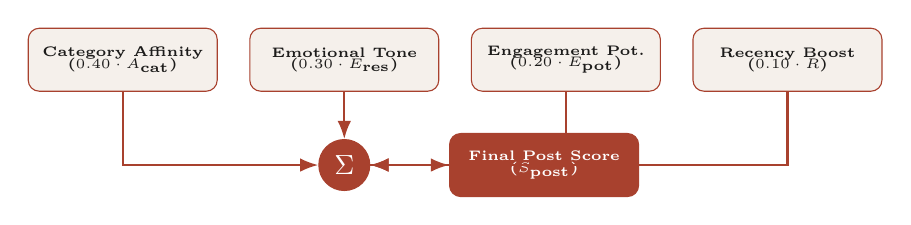
\begin{tikzpicture}[
        node/.style={draw, rounded corners, minimum width=2.4cm, minimum height=0.8cm, align=center, font=\tiny\bfseries, fill=echobg, draw=echored, text=echoink},
        sum/.style={circle, draw=echored, fill=echored, text=white, font=\bfseries, inner sep=3pt},
        line/.style={-Latex, thick, echored}
    ]
        \node (a) [node] {Category Affinity\\[-2pt]\tiny ($0.40 \cdot A_{\text{cat}}$)};
        \node (e) [node, right=0.4cm of a] {Emotional Tone\\[-2pt]\tiny ($0.30 \cdot E_{\text{res}}$)};
        \node (p) [node, right=0.4cm of e] {Engagement Pot.\\[-2pt]\tiny ($0.20 \cdot E_{\text{pot}}$)};
        \node (r) [node, right=0.4cm of p] {Recency Boost\\[-2pt]\tiny ($0.10 \cdot R$)};
        
        \node (plus) [sum, below=0.6cm of e] {$\Sigma$};
        \node (score) [node, fill=echored, text=white, right=1cm of plus] {Final Post Score\\[-2pt]\tiny ($S_{\text{post}}$)};
        
        \draw [line] (a) |- (plus);
        \draw [line] (e) -- (plus);
        \draw [line] (p) |- (plus);
        \draw [line] (r) |- (plus);
        \draw [line] (plus) -- (score);
    \end{tikzpicture}
    \caption{Diagram 7: Real-time Mathematical Scoring Engine Pipeline.}
    \label{fig:scoring_pipeline}
\end{figure}

\vspace{4pt}
\begin{center}
\renewcommand{\arraystretch}{1.3}
\begin{tabularx}{0.94\textwidth}{>{\bfseries}l X l}
\toprule
Term & Definition & Range \\
\midrule
$A_{\text{cat}}$ & Category affinity normalised to the user's highest-liked category & $[0,\,1]$ \\
$E_{\text{res}}$ & Emotional tone resonance normalised to the dominant emotion & $[0,\,1]$ \\
$E_{\text{pot}}$ & Engagement potential from content metadata, divided by 10 & $[0,\,1]$ \\
$R$ & Recency boost: $\max(0.1,\;1 - h/24)$, where $h$ = hours since publish & $[0.1,\,1]$ \\
\bottomrule
\end{tabularx}
\end{center}

At session start, $A_{\text{cat}}$ and $E_{\text{res}}$ both return $0.5$, ensuring ranking is driven by content metadata alone, not artificially biased before the student makes a choice.

\phantomsection
\section*{Appendix B: Module Architecture \& Complete File Map}
\addcontentsline{toc}{section}{Appendix B: Module Architecture \& Complete File Map}

\begin{center}
\renewcommand{\arraystretch}{1.25}
\begin{tabular}{ll}
\toprule
\textbf{File} & \textbf{Role \& System Description} \\
\midrule
\texttt{index.html}      & Feed Simulator entry point \\
\texttt{game.html}       & Echo Escape Arena + Teacher Facilitation Guide \\
\texttt{toolkit.html}    & Agency Toolkit (20-item interactive audit checklist) \\
\texttt{dashboard.html}  & Educator Impact Command Center \\
\texttt{print-game.html} & Offline printable card game worksheet (Plan B) \\
\texttt{print-report.html}& Offline printable student reflection report (Plan B) \\
\texttt{render.yaml}     & Render Blueprint automated deployment specification \\
\midrule
\texttt{css/styles.css}  & Primary component theme \& responsive layout \\
\texttt{css/globals.css} & Global typography, CSS custom properties, color palette \\
\texttt{css/icon\_system.css} & Custom SVG \& FontAwesome icon definitions \\
\midrule
\texttt{js/engine.js}    & Live scoring formula $S_{\text{post}}$ \& student state manager \\
\texttt{js/feed.js}      & Feed renderer \& dwell-time \texttt{IntersectionObserver} \\
\texttt{js/impact.js}    & Echo chamber alert modal controller \\
\texttt{js/diversity.js} & Feed diversity calculation ($D < 0.35$) engine \\
\texttt{js/telemetry.js} & Zero-PII aggregate metrics collector \\
\texttt{js/i18n.js}      & Multi-language localization string provider \\
\bottomrule
\end{tabular}
\end{center}

\end{document}
